\chapter{Prezentacja warstwy użytkowej}
Projekt sklepu został w całości zrealizowany jako aplikacja konsolowa. Oznacza to, że zarówno logika działania programu oraz jej wygląd zostały napisane w języku C\#. Jest to także jednoznaczne z tym, że poruszanie się po programie przez użytkownika odbywa się w konsoli bez dodatkowego interfejsu graficznego, przy pomocy jedynie klawiatury.\newline

Poniżej zostaną przedstawione zrzuty ekranu z najważniejszych funkcjonalności w programie, aby zaprezentować w ten sposób wygląd oraz pogląd działania aplikacji.\newline

Po uruchomieniu aplikacji pierwszym ekranem jest ekran powitalny, który jednocześnie jest miejscem wyboru roli użytkownika, który będzie korzystał z programu. Z programu można korzystać jako sprzedawca lub klient.\newline

\section{Sprzedawca}

\begin{figure}[H]
	\centering
		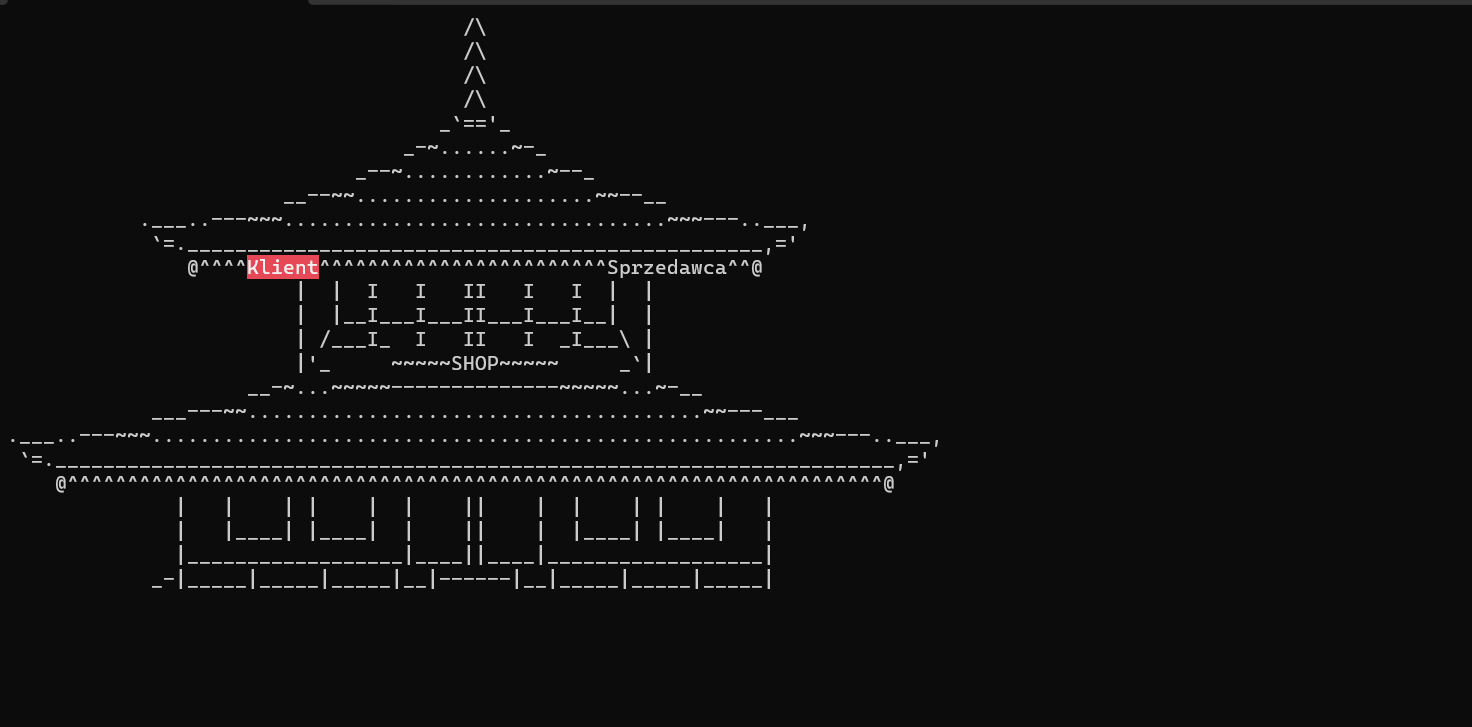
\includegraphics[width=15cm]{screeny/ekran_start.png}
	\caption{\footnotesize Wybór roli użytkownika}
	\label{fig:plotend}
\end{figure}

Po wyborze roli pojawia się ekran, w którym należy zdecydować pomiędzy zalogowaniem się lub rejestracją. Wygląd tych ekranów jest identyczny zarówno dla sprzedawcy jak i klienta. W zależności od wyboru wyświetlają się formularze gdzie kolejno należy podawać kolejne informacje. W przypadku rejestracji w systemie tworzy się konto użytkownika z rolą odpowiadającą wcześniejszemu wyborowi.

\begin{figure}[H]
    \centering
		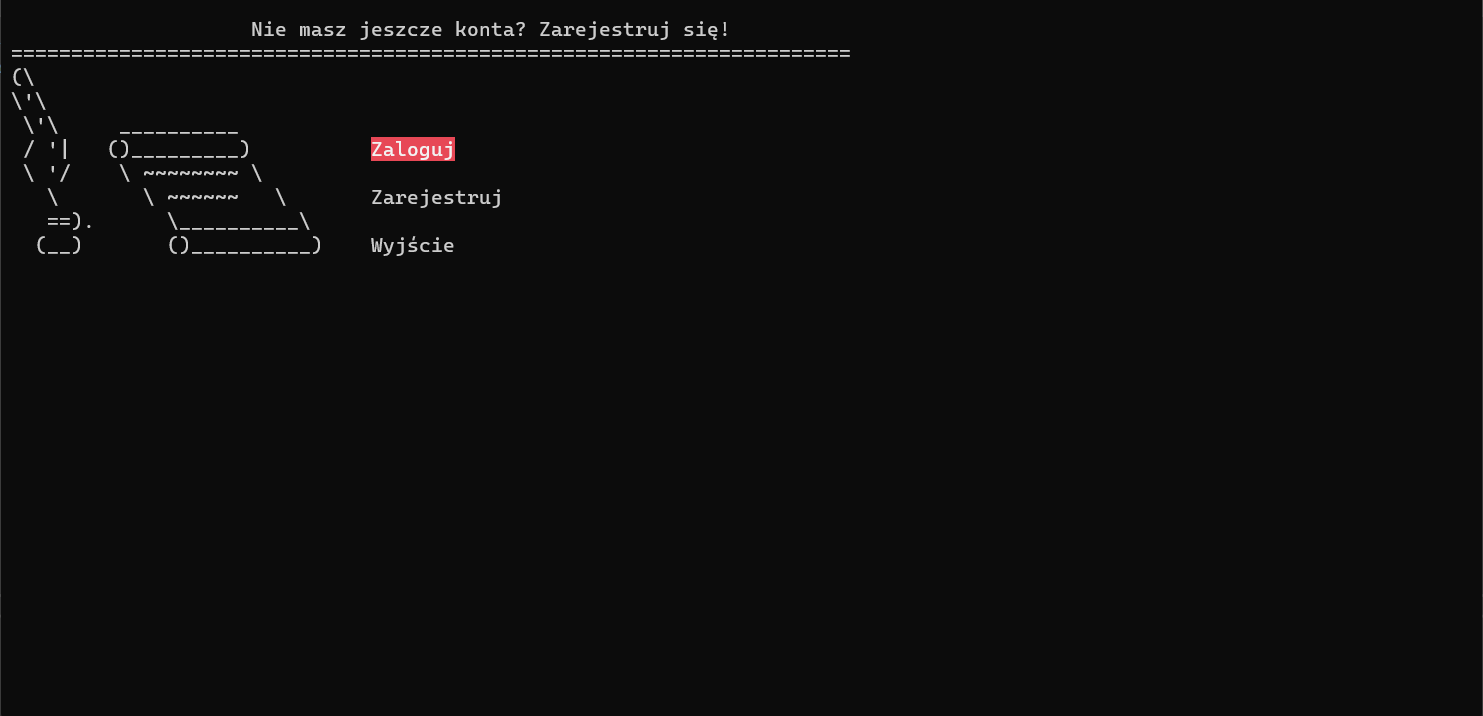
\includegraphics[width=15cm]{screeny/logowanie_sprzedawca.png}
	\caption{\footnotesize Ekran logowania i rejestracji}
	\label{fig:plotend}
\end{figure}

Logując się do aplikacji jako sprzedawca ma on do wyboru opcje widoczne na \textit{Rysunku 5.3}.

\begin{figure}[H]
	\centering
		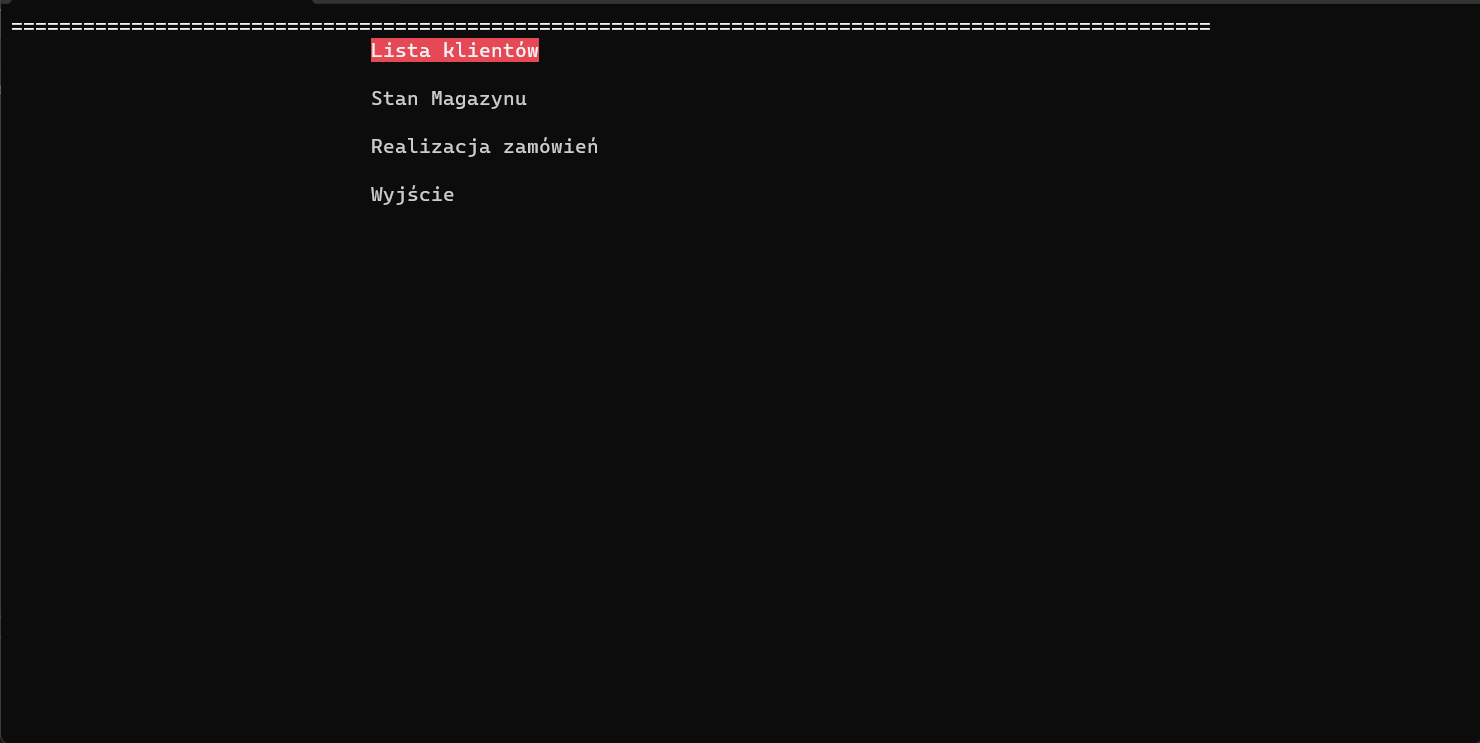
\includegraphics[width=15cm]{screeny/sprzedawca_menu.png}
	\caption{\footnotesize Menu sprzedawcy}
	\label{fig:plotend}
\end{figure}

Po przejściu do opcji \textit{Lista klientów}, sprzedawca ma możliwość usunięcia klienta po adresie e-mail. Na liście wyświetlają się tylko użytkownicy z rolą klienta. Widać ich podstawowe dane personalne oraz liczbę zamówień złożonych w systemie. Ekran ten zaprezentowany został na \textit{Rysunku 5.4}.

\begin{figure}[H]
	\centering
		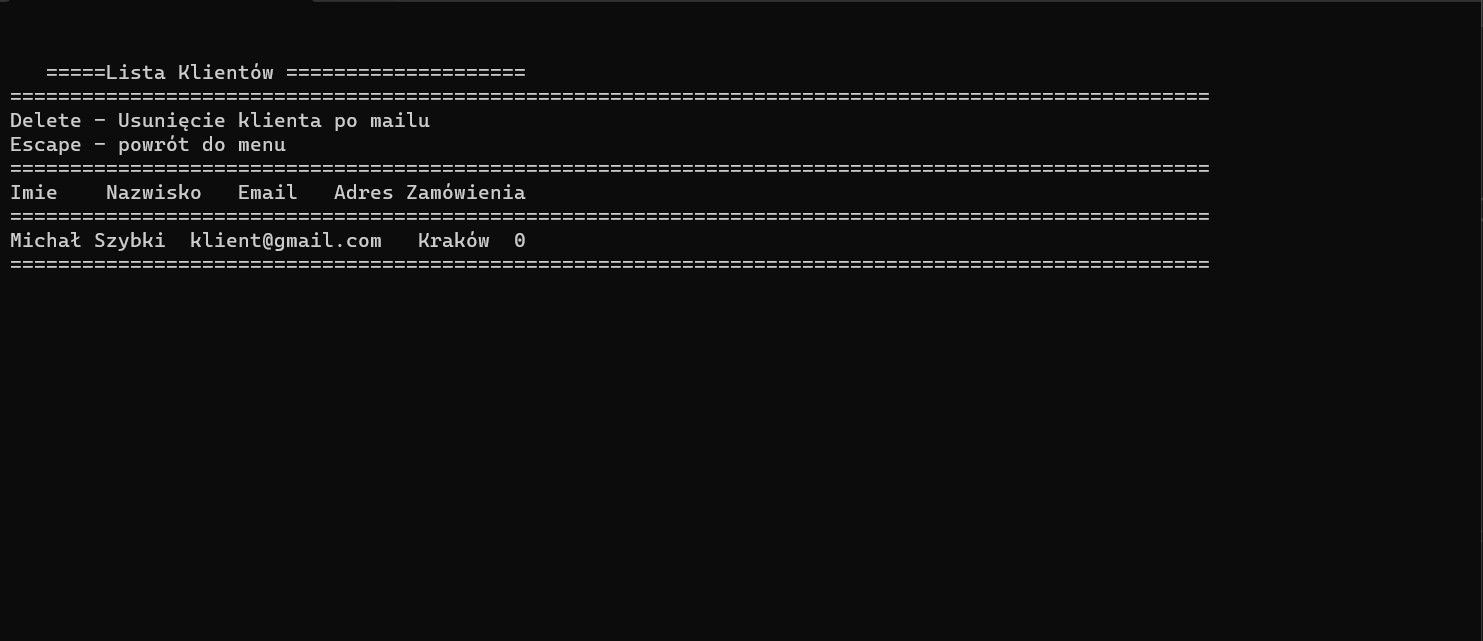
\includegraphics[width=15cm]{screeny/lista_klientow.png}
	\caption{\footnotesize Lista klientów}
	\label{fig:plotend}
\end{figure}

Kolejną możliwą opcją jest wyświetlenie stanu magazynu, czyli wszystkich dostępnych produktów w sklepie. Ponadto, w tym menu można również dodać nowy produkt, usunąć go lub edytować. Możliwe jest również posortowanie na liście produktów po nazwie. Jeśli sprzedawca uzna, że chce na przykład wydrukować daną listę lub ją wyeksportować, ma możliwość wygenerowania pliku pdf z dostępnymi w sklepie towarami.

\begin{figure}[H]
	\centering
		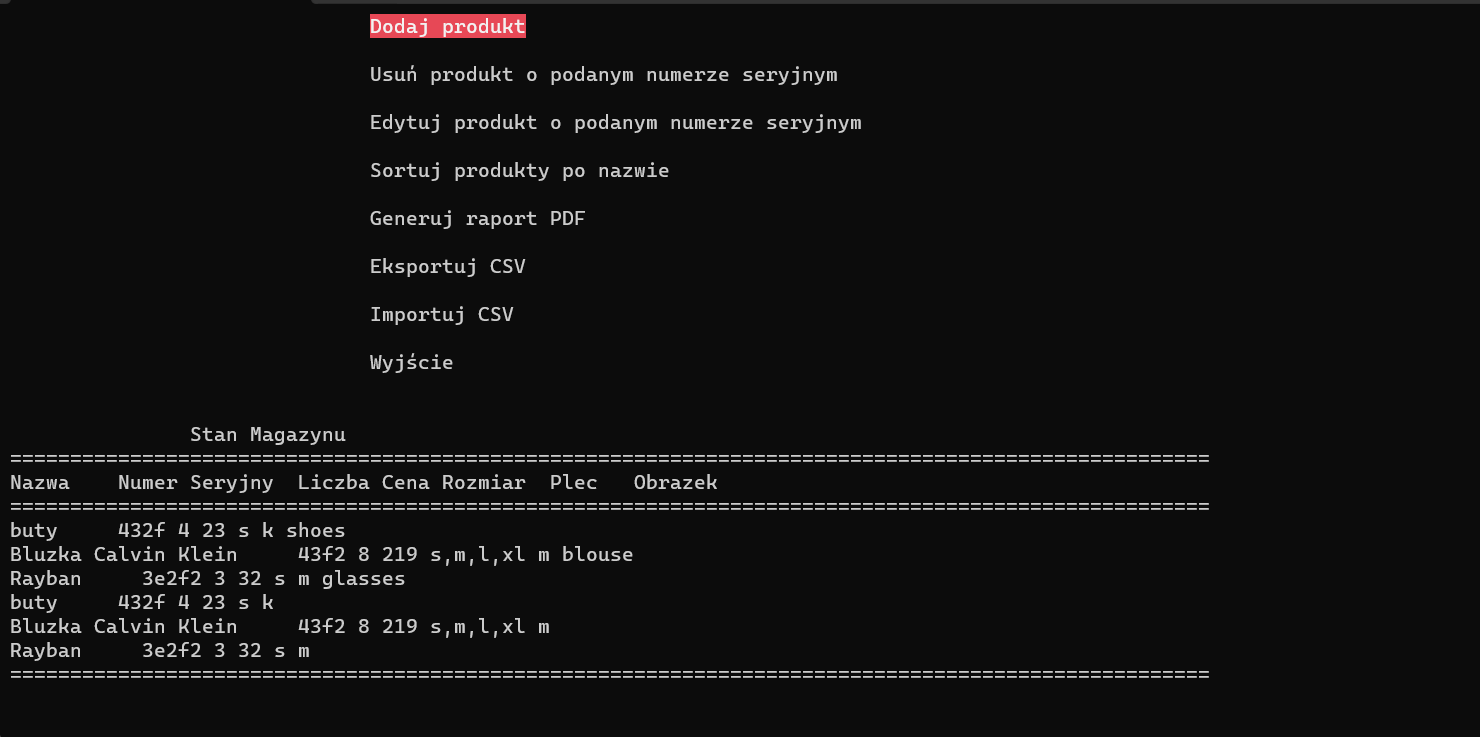
\includegraphics[width=15cm]{screeny/lista_produktow_sprz.png}
	\caption{\footnotesize Menu stan magazynu}
	\label{fig:plotend}
\end{figure}

W otatniej zakładce od strony sprzedawcy, mianowicie \textit{Realizacja zamówień}, wyświetlane są wszystkie zamówienia w systemie zarówno te zrealizowane jak i te, które dopiero zostały złożone. Sprzedawca może usunąć wybrane zamówienie z listy zamówień lub zrealizować zamówienie. Metoda ta zmienia status zamówienia z \textit{złożone} na \textit{zrealizowane}.

\begin{figure}[H]
	\centering
		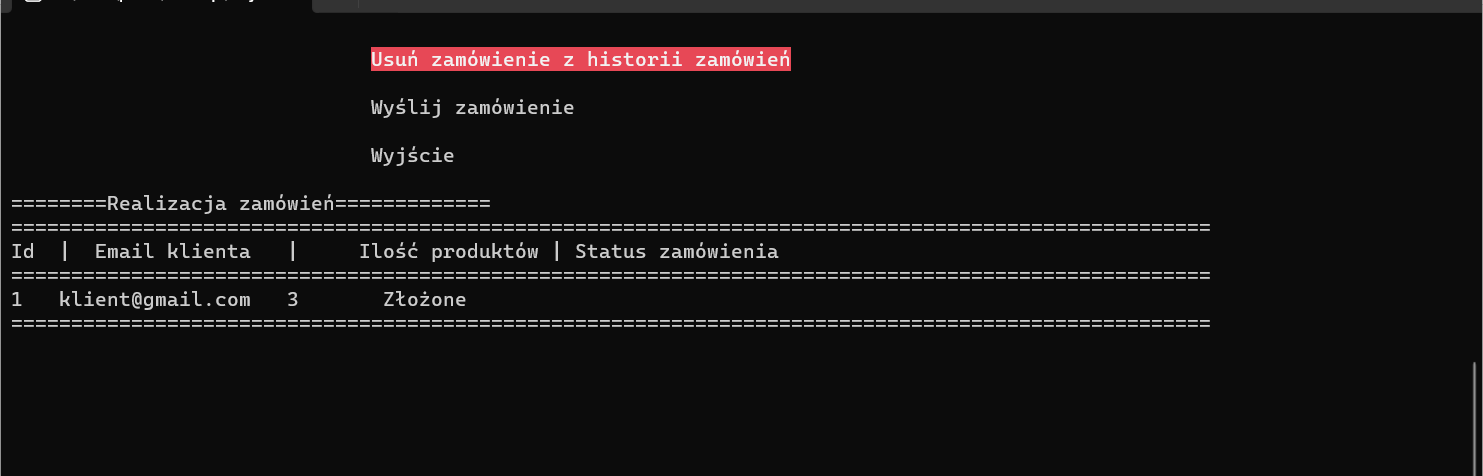
\includegraphics[width=15cm]{screeny/zamowienia_sprzedawca.png}
	\caption{\footnotesize Menu realizacja zamówień}
	\label{fig:plotend}
\end{figure}

\section{Klient}

Klient po poprawnym zalogowaniu do systemu, oprócz wiadomości powitalnej w lewym górnym rogu aplikacji ma do wyboru jedną z kilku opcji widocznych na \textit{Rysunku 5.7}. 

\begin{figure}[H]
	\centering
		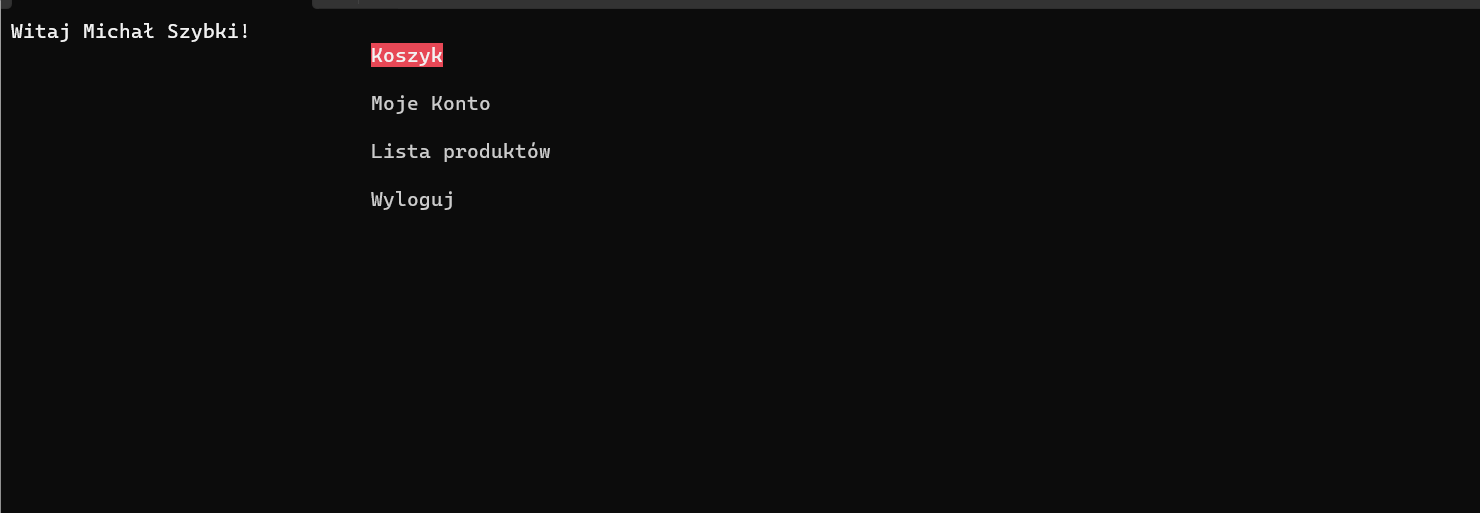
\includegraphics[width=15cm]{screeny/klient_menu.png}
	\caption{\footnotesize Menu klienta}
	\label{fig:plotend}
\end{figure}

Aby jednak w pierwszych dwóch pozycjach z menu wyświetliły się jakieś dane w przypadku nowo utoworzonego konta, należy najpierw przejść do opcji \textit{Lista produktów}. Aplikacja przekieruje użytkownika do widoku z dostępnymi produktami w sklepie, które następnie można sortować lub wyszukać po nazwie. 

\begin{figure}[H]
	\centering
		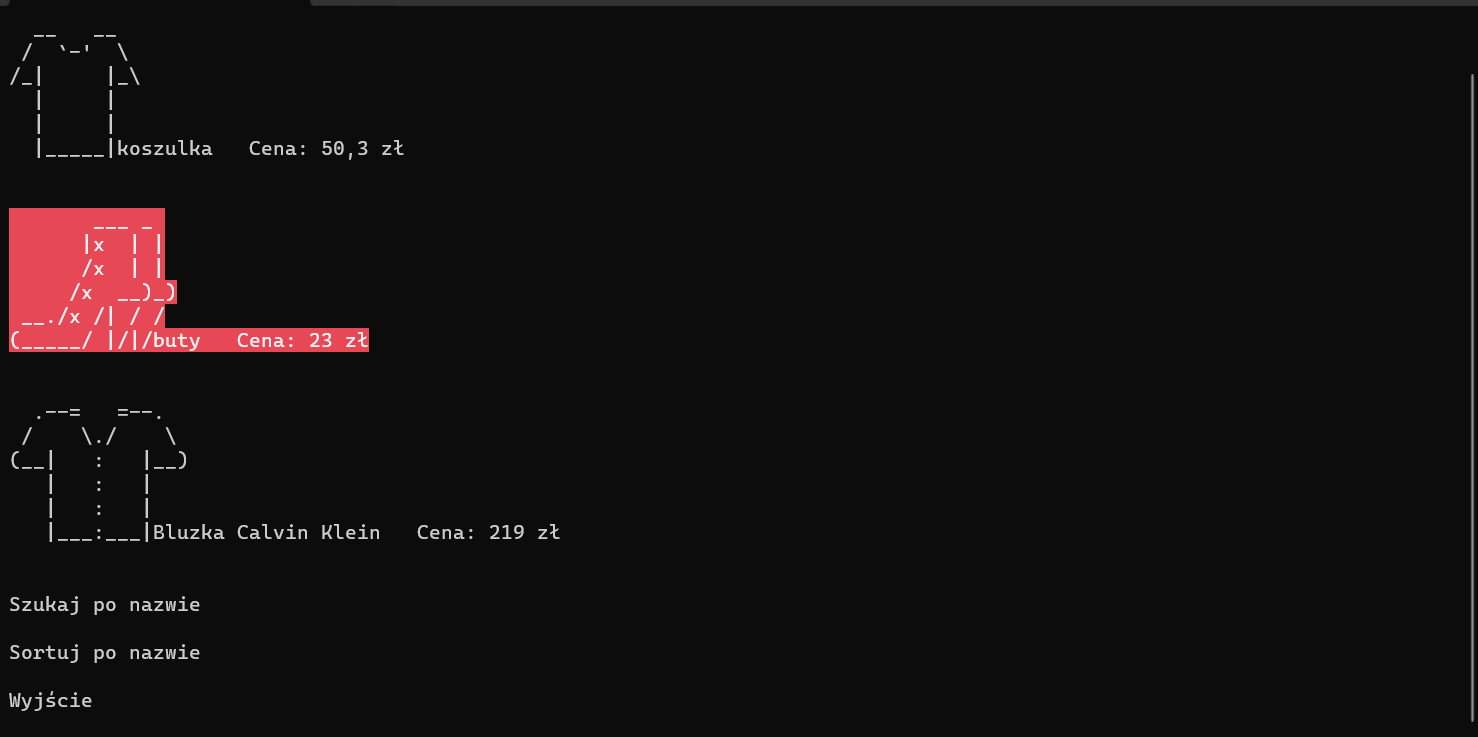
\includegraphics[width=15cm]{screeny/sklep_klient.png}
	\caption{\footnotesize Przeglądanie listy produktów w menu klienta}
	\label{fig:plotend}
\end{figure}

Rezultat wyszukiwania produktu po nazwie z frazą \textit{calvin} widoczny na \textit{Rysunku 5.9}.
	
\begin{figure}[H]
	\centering
		
\includegraphics[width=15cm]{screeny/szukaj.png}
	\caption{\footnotesize Wyszukiwanie produktu po nazwie}
	\label{fig:plotend}
\end{figure}

Po wybraniu upatrzonego produktu, użytkownik może wybrać rozmiar oraz ilość sztuk. Jeśli wszystkie parametry zostały wybrane poprawnie, klient może dodać produkt do koszyka.

\begin{figure}[H]
	\centering
		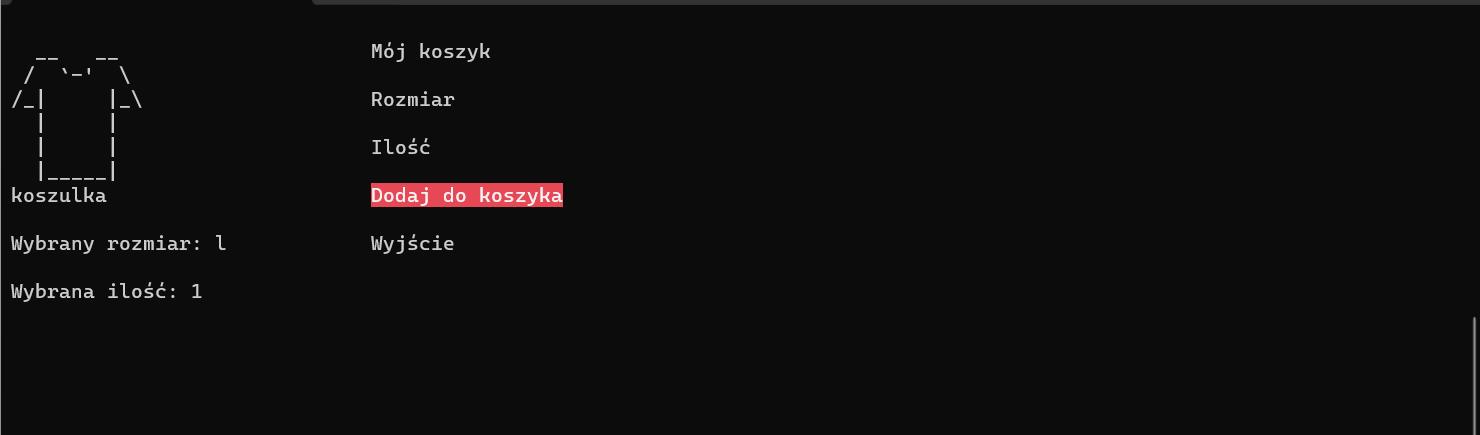
\includegraphics[width=15cm]{screeny/dodawanie_produktu_do_koszyka.png}
	\caption{\footnotesize Dodawanie produktu do koszyka}
	\label{fig:plotend}
\end{figure}

W koszyku znajdują się produkty, które klient dodał tam podczas działania aplikacji. Są one w nim widoczne tylko na czas działania aplikacji, czyli na czas sesji. W koszyku wyświetlana jest zsumowana liczba wszystkich produktów oraz zsumowana kwota zakupów. Klient widzi również dane do wysyłki. Są to dane podane podczas procesu rejestracji. W tym miejscu klient może jeszcze usunąć wybrany produkt z koszyka podając jego numer z listy w koszyku. Użytkownik może również wybrać opcję potwierdzenia zakupów, która utworzy zamówienie w systemie, aktualizując liczbę produktów w bazie danych oraz wyczyści koszyk klienta.

\begin{figure}[H]
	\centering
		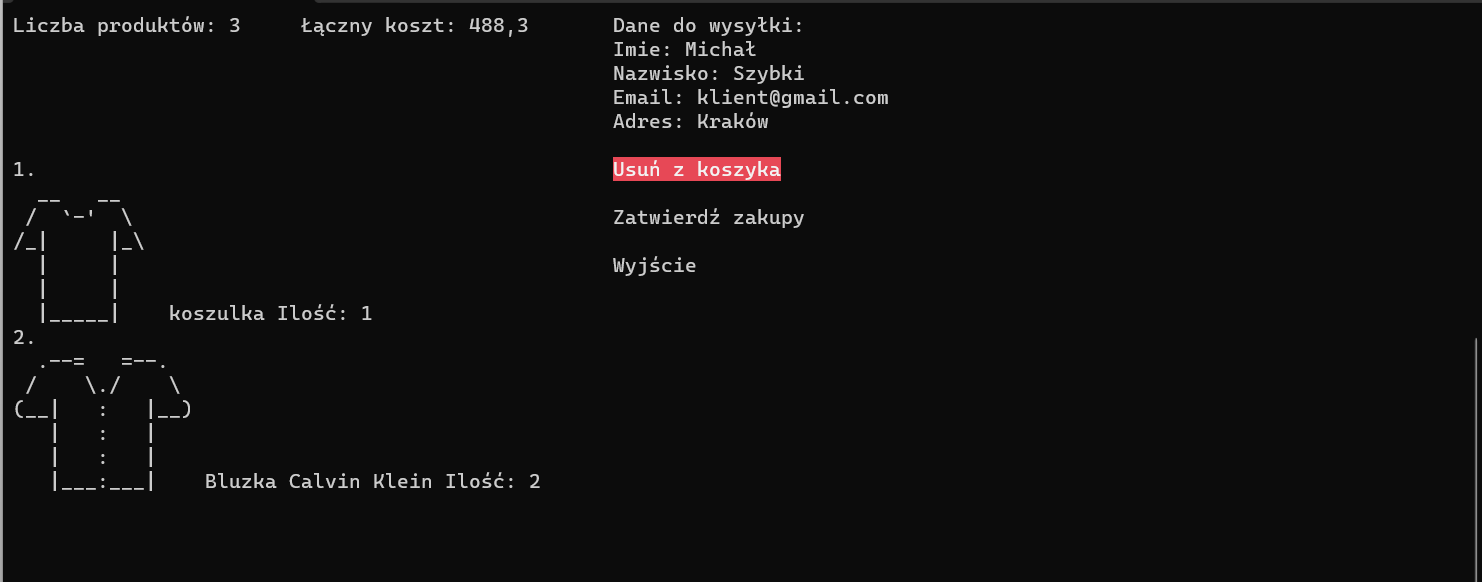
\includegraphics[width=15cm]{screeny/koszyk.png}
	\caption{\footnotesize Podgląd koszyka klienta}
	\label{fig:plotend}
\end{figure}

Ostatnią opcją, która nie została jeszcze opisana z menu klienta z \textit{Rysunku 5.7}, jest zakładka \textit{Moje konto}. Klient może tu zobaczyć swoje dane, w tym hasło. Co więcej, opcja ta wyświetla listę zamówień złożonych przez klienta w sklepie. Klient może wybrać konkretne zamówienie z listy i podejrzeć jakie produkty kupił w danym zamówieniu.

\begin{figure}[H]
	\centering
		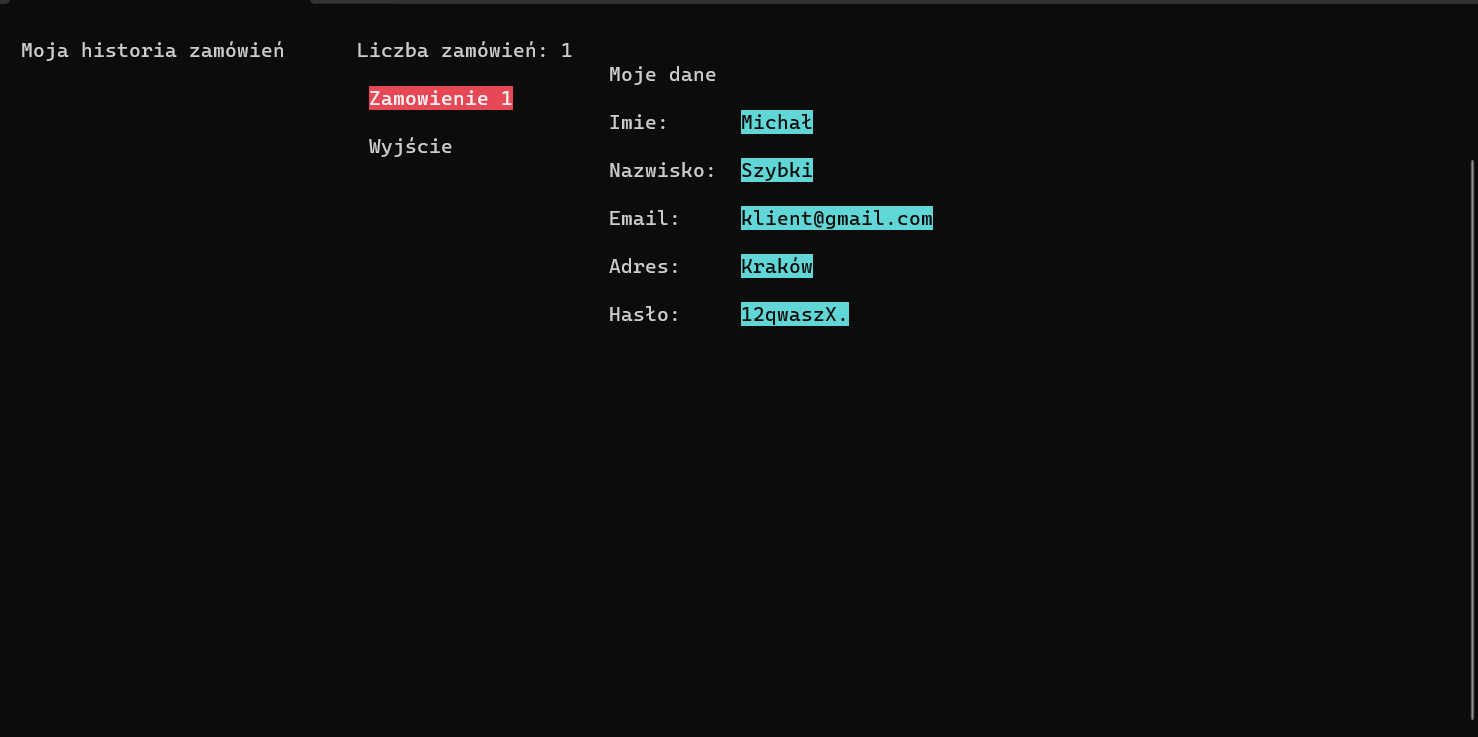
\includegraphics[width=15cm]{screeny/historia_klienta.png}
	\caption{\footnotesize Historia zamówień klienta oraz dane jego konta}
	\label{fig:plotend}
\end{figure}